% GroundFall-US preprint. Every number comes from numbers.tex and tables/*.tex,
% which code/09_paper_stats.py generates from the released data. Do not type numbers.
\documentclass[letterpaper,twocolumn,10pt]{article}
\usepackage[letterpaper,textwidth=7in,textheight=9.25in,top=0.75in,columnsep=0.33in]{geometry}
\usepackage{times}
\usepackage[T1]{fontenc}
\usepackage{helvet}
\usepackage{courier}
\usepackage[hyphens]{url}
\usepackage{graphicx}
\usepackage{booktabs}
\usepackage{tabularx}
\usepackage{array}
\usepackage{amsmath}
\usepackage{enumitem}
\usepackage[authoryear,round]{natbib}
\usepackage{titlesec}
\usepackage{caption}
\usepackage{float}
\usepackage{xcolor}
\usepackage[hidelinks]{hyperref}
\urlstyle{rm}
\frenchspacing
\setlength{\parindent}{10pt}
\setlength{\bibsep}{2pt}
\renewcommand{\bibfont}{\small}
\setlength{\bibhang}{1em}
\captionsetup{font=small,labelsep=colon,skip=4pt}
\titleformat{\section}{\centering\large\bfseries}{}{0pt}{}
\titlespacing*{\section}{0pt}{10pt}{4pt}
\titleformat{\subsection}{\normalsize\bfseries}{}{0pt}{}
\titlespacing*{\subsection}{0pt}{8pt}{3pt}
\titleformat{\paragraph}[runin]{\normalsize\bfseries}{}{0pt}{}[.]
\titlespacing*{\paragraph}{0pt}{4pt}{0.5em}
\setlist{itemsep=1pt,topsep=3pt,leftmargin=*}
\newcolumntype{L}{>{\raggedright\arraybackslash}X}
% Generated by code/09_paper_stats.py from the GroundFall-US outputs. Do not edit.
\newcommand{\CFRAll}{0.53}
\newcommand{\CFRCSurf}{17.1}
\newcommand{\CFRCUG}{1.3}
\newcommand{\CFRGF}{1.71}
\newcommand{\CFRMSurf}{12.7}
\newcommand{\CFRMUG}{3.0}
\newcommand{\CFRRatio}{3.2}
\newcommand{\CFRSurf}{14.9}
\newcommand{\CFRSurfVsUG}{10}
\newcommand{\CFRUG}{1.5}
\newcommand{\CandRatio}{2.5}
\newcommand{\ComMetal}{22}
\newcommand{\ComNonmetal}{8}
\newcommand{\ComSandGravel}{14}
\newcommand{\ComStone}{48}
\newcommand{\FCountFirstCSurf}{2}
\newcommand{\FCountFirstCUG}{25}
\newcommand{\FCountFirstMSurf}{3}
\newcommand{\FCountFirstMUG}{5}
\newcommand{\FCountLastCSurf}{1}
\newcommand{\FCountLastCUG}{9}
\newcommand{\FCountLastMSurf}{1}
\newcommand{\FCountLastMUG}{7}
\newcommand{\FRateAllCSurf}{0.7}
\newcommand{\FRateAllCUG}{5.5}
\newcommand{\FRateAllMSurf}{0.2}
\newcommand{\FRateAllMUG}{5.0}
\newcommand{\FRateDropCSurf}{21}
\newcommand{\FRateDropCUG}{56}
\newcommand{\FRateDropMSurf}{73}
\newcommand{\FRateDropMUG}{8}
\newcommand{\FRateFirstCSurf}{0.6}
\newcommand{\FRateFirstCUG}{7.0}
\newcommand{\FRateFirstMSurf}{0.4}
\newcommand{\FRateFirstMUG}{6.0}
\newcommand{\FRateHiFirstCSurf}{2.2}
\newcommand{\FRateHiFirstCUG}{10.3}
\newcommand{\FRateHiFirstMSurf}{1.1}
\newcommand{\FRateHiFirstMUG}{14.0}
\newcommand{\FRateHiLastCSurf}{2.7}
\newcommand{\FRateHiLastCUG}{5.9}
\newcommand{\FRateHiLastMSurf}{0.6}
\newcommand{\FRateHiLastMUG}{11.3}
\newcommand{\FRateLastCSurf}{0.5}
\newcommand{\FRateLastCUG}{3.1}
\newcommand{\FRateLastMSurf}{0.1}
\newcommand{\FRateLastMUG}{5.5}
\newcommand{\FRateLoFirstCSurf}{0.1}
\newcommand{\FRateLoFirstCUG}{4.5}
\newcommand{\FRateLoFirstMSurf}{0.1}
\newcommand{\FRateLoFirstMUG}{1.9}
\newcommand{\FRateLoLastCSurf}{0.0}
\newcommand{\FRateLoLastCUG}{1.4}
\newcommand{\FRateLoLastMSurf}{0.0}
\newcommand{\FRateLoLastMUG}{2.2}
\newcommand{\FRateUGMetal}{5.2}
\newcommand{\FRateUGNonmetal}{3.2}
\newcommand{\FRateUGStone}{6.5}
\newcommand{\FRatioMNMUGvsSurf}{25}
\newcommand{\FRatioUGCoalVsSurfMNM}{28}
\newcommand{\HoursCSurf}{1.51}
\newcommand{\HoursCUG}{1.87}
\newcommand{\HoursMSurf}{4.16}
\newcommand{\HoursMUG}{0.52}
\newcommand{\HoursMatchPct}{99.65}
\newcommand{\InjIDMUG}{127}
\newcommand{\InjNVMUG}{90}
\newcommand{\KhDiffPct}{3.2}
\newcommand{\KhFatal}{50}
\newcommand{\KhN}{8,572}
\newcommand{\KhNoInj}{5,188}
\newcommand{\KhNoInjDiffPct}{0.3}
\newcommand{\LastDate}{09/23/2026}
\newcommand{\MineMatchPct}{100.0}
\newcommand{\ModeCollapseMechanismUnstated}{21}
\newcommand{\ModePlanar}{1}
\newcommand{\ModeRaveling}{8}
\newcommand{\ModeRockfall}{41}
\newcommand{\ModeRotationalSlide}{2}
\newcommand{\ModeToppling}{2}
\newcommand{\ModeUnspecified}{16}
\newcommand{\ModeWedge}{1}
\newcommand{\NAllAccidents}{275,220}
\newcommand{\NAllFatal}{1,215}
\newcommand{\NAllInjury}{228,860}
\newcommand{\NCSurf}{161}
\newcommand{\NCUG}{28,034}
\newcommand{\NCand}{226}
\newcommand{\NCandFatal}{13}
\newcommand{\NCandMach}{48}
\newcommand{\NCandPH}{52}
\newcommand{\NCoded}{92}
\newcommand{\NCodedFatal}{10}
\newcommand{\NCollapseFatal}{6}
\newcommand{\NEquipment}{44}
\newcommand{\NExcavator}{16}
\newcommand{\NFace}{2,379}
\newcommand{\NFaceCSurf}{161}
\newcommand{\NFaceMSurf}{92}
\newcommand{\NFatCSurf}{14}
\newcommand{\NFatCUG}{109}
\newcommand{\NFatMSurf}{10}
\newcommand{\NFatMUG}{29}
\newcommand{\NFatalCoal}{562}
\newcommand{\NFatalMNM}{653}
\newcommand{\NGF}{29,851}
\newcommand{\NGFContractor}{719}
\newcommand{\NGFFatal}{162}
\newcommand{\NGFInjury}{9,465}
\newcommand{\NGFNoInjury}{20,327}
\newcommand{\NInjCSurf}{82}
\newcommand{\NInjCUG}{8,343}
\newcommand{\NInjMSurf}{79}
\newcommand{\NInjMUG}{958}
\newcommand{\NLoader}{11}
\newcommand{\NMSurf}{92}
\newcommand{\NMUG}{1,561}
\newcommand{\NMechanismNamed}{6}
\newcommand{\NNoInjCSurf}{78}
\newcommand{\NNoInjCUG}{19,643}
\newcommand{\NNoInjCoded}{12}
\newcommand{\NNoInjMSurf}{12}
\newcommand{\NNoInjMUG}{594}
\newcommand{\NPatterns}{46}
\newcommand{\NRoof}{27,472}
\newcommand{\NStatesCSurf}{26}
\newcommand{\NStatesCUG}{17}
\newcommand{\NStatesMSurf}{55}
\newcommand{\NStatesMUG}{39}
\newcommand{\NSurfFat}{24}
\newcommand{\NSurfInj}{161}
\newcommand{\PctEquipment}{48}
\newcommand{\PctGFNoInjury}{68.1}
\newcommand{\PctGFofFatal}{13.3}
\newcommand{\PctGFofFatalCoal}{21.9}
\newcommand{\PctGFofFatalMNM}{6.0}
\newcommand{\PctGFofInjury}{4.1}
\newcommand{\PctMechanismNamed}{7}
\newcommand{\PctNoInjCSurf}{48.4}
\newcommand{\PctNoInjCUG}{70.1}
\newcommand{\PctNoInjMSurf}{13.0}
\newcommand{\PctNoInjMUG}{38.1}
\newcommand{\PctTrigAny}{21}
\newcommand{\PctUnspecified}{17}
\newcommand{\RateAllCSurf}{0.0090}
\newcommand{\RateAllCUG}{0.829}
\newcommand{\RateAllMSurf}{0.0032}
\newcommand{\RateAllMUG}{0.318}
\newcommand{\RateDropCSurf}{73}
\newcommand{\RateDropCUG}{37}
\newcommand{\RateDropMSurf}{74}
\newcommand{\RateDropMUG}{59}
\newcommand{\RateFirstCSurf}{0.0140}
\newcommand{\RateFirstCUG}{0.857}
\newcommand{\RateFirstMSurf}{0.0046}
\newcommand{\RateFirstMUG}{0.412}
\newcommand{\RateIDMUG}{1.36}
\newcommand{\RateLastCSurf}{0.0038}
\newcommand{\RateLastCUG}{0.541}
\newcommand{\RateLastMSurf}{0.0012}
\newcommand{\RateLastMUG}{0.170}
\newcommand{\RateNVMUG}{0.17}
\newcommand{\RateUGMetal}{0.391}
\newcommand{\RateUGNonmetal}{0.210}
\newcommand{\RateUGStone}{0.249}
\newcommand{\RatioUGCoalVsSurfMNM}{259}
\newcommand{\RulesVersion}{1.0}
\newcommand{\TopThreeCUG}{WV, KY, IL}
\newcommand{\TopThreeShareCSurf}{62}
\newcommand{\TopThreeShareCUG}{70}
\newcommand{\TopThreeShareMSurf}{23}
\newcommand{\TopThreeShareMUG}{46}
\newcommand{\TrigAny}{19}
\newcommand{\TrigBlasting}{6}
\newcommand{\TrigScaling}{6}
\newcommand{\TrigWater}{8}
\newcommand{\YRateCoalUndergroundTwoZeroTwoFive}{0.38}
\newcommand{\YRateCoalUndergroundTwoZeroZeroZero}{1.18}
\newcommand{\YRateMNMUndergroundTwoZeroTwoFive}{0.13}
\newcommand{\YRateMNMUndergroundTwoZeroZeroZero}{0.62}

\makeatletter\newcommand{\tablefile}[1]{\@@input #1 }\makeatother

\title{\Large\bfseries GroundFall-US: An Open Dataset of Ground-Failure Incidents at U.S. Mines, 2000--2026, with Rates and a Failure-Mode Coding Layer}
\author{\normalsize\bfseries Lukman Alabede\textsuperscript{\rm 1}, Kayode Komolafe\textsuperscript{\rm 2}\\[4pt]
\normalsize\textsuperscript{1}Independent Researcher, Safford, Arizona, USA\\
\normalsize\textsuperscript{2}Mining Engineering Department, Colorado School of Mines, Golden, Colorado, USA\\
\normalsize lukmanademola081@gmail.com, komolafe@mines.edu}
\date{}

\begin{document}
\maketitle

\begin{abstract}
\noindent Falls of roof, rib, face, highwall, and slope remain among the most lethal hazards in U.S. mining, yet the federal record of these events is spread across separate files that are hard to join and do not record how the ground failed. We present GroundFall-US, an open, documented dataset that joins the Mine Safety and Health Administration (MSHA) Accidents, Mines, and yearly Employment/Production files into \NGF{} ground-failure records from 2000 to 2026, with injury and fatality rates per hour worked by sector, mine type, commodity, and state, and a rule-based failure-mode layer (rockfall, raveling, planar, wedge, toppling, rotational slide; blasting, water, and scaling triggers) for surface metal and nonmetal narratives. Ground failures account for \PctGFofInjury\% of reportable injuries but \PctGFofFatal\% of deaths in MSHA's accident file. They are rare at surface mines but lethal there: \CFRSurf\% of surface ground-failure injuries were fatal, against \CFRCUG\% in underground coal. Injury rates fell in every setting, but the fatality rate at underground metal and nonmetal mines did not fall with them. At surface metal and nonmetal mines, \PctUnspecified\% of narratives name no mechanism, only \PctMechanismNamed\% name a structurally controlled one, and MSHA's own classification misses comparable events: screening other categories yields \NCand{} candidate ground failures, \CandRatio{} times the number selected. We release the data, code, rules, and source fingerprints under open licenses, and recommend structured ground-failure fields in federal accident reporting as the basis for early warning under 30 CFR 56.3130.
\end{abstract}

\section{Introduction}
When rock or soil gives way at a mine, the people nearest the face, wall, or bench have seconds or less to react. U.S. regulations address this hazard directly: at surface metal and nonmetal mines, 30 CFR 56.3130 requires that mining methods maintain the stability of walls, banks, and slopes where persons work or travel \citep{CFR563130}, and companion standards cover scaling, inspection, and ground support. Every operator must report accidents, injuries, and certain non-injury events, including unplanned roof falls, to MSHA under 30 CFR Part 50 \citep{CFRPart50}. MSHA publishes those reports as open data, refreshed weekly \citep{MSHAOGD}.

The record exists, but it is not easy to use for ground control. The accident reports, the list of mines, and the hours each mine worked live in three separate files with different keys and column names. The accident file classifies each event by the circumstance that most directly contributed, so ``fall of face, rib, pillar, side, highwall'' and ``fall of roof or back'' can be counted, but it does not record whether a highwall failed as a wedge, a toppling column, or a slump, or what set it off. That information exists only in a free-text narrative of at most 384 characters. Studies of ground falls have therefore centred on underground coal, where roof and rib falls dominate and NIOSH has tracked trends for decades \citep{MarkPappasBarczak2009,PappasMark2012,Khademian2022}. Surface walls and slopes, the subject of 56.3130, have received less systematic national attention.

We ask: \textbf{\textit{Where, at which kinds of U.S. mines, and how do ground failures that injure miners occur, and what does the federal record allow us to say about the failure mechanism?}} We answer with GroundFall-US, an open dataset built entirely from public MSHA files, and report three findings:
\begin{enumerate}
\item \textbf{Ground failures are a small share of injuries but a large share of deaths, and surface failures are the deadliest.} They are \PctGFofInjury\% of reportable injuries but \PctGFofFatal\% of fatalities in MSHA's accident file for 2000--2026 (\PctGFofFatalCoal\% in coal). A ground-failure injury is \CFRRatio{} times as likely to be fatal as the average injury, and at surface mines \CFRSurf\% are fatal.
\item \textbf{Injury rates have fallen everywhere, but not evenly, and not for deaths.} The underground coal injury rate fell \RateDropCUG\% between 2000--04 and 2020--25. At underground metal and nonmetal mines the injury rate fell \RateDropMUG\%, while the fatality rate stayed at \FRateFirstMUG{} and \FRateLastMUG{} deaths per 100 million hours in the first and last periods. Injuries concentrate in a few states: \TopThreeCUG{} account for \TopThreeShareCUG\% of underground coal ground-failure injuries.
\item \textbf{The federal record rarely says how surface walls fail, and sometimes does not say that they failed.} Of \NCoded{} surface metal and nonmetal narratives, rules flag \ModeRockfall{} as rockfall and \ModeCollapseMechanismUnstated{} as wall or bank collapse with no mechanism stated; only \NMechanismNamed{} name a structurally controlled mechanism, and \PctTrigAny\% name any trigger. A screen of other MSHA categories finds \NCand{} further narratives that read as ground failures, including \NCandFatal{} fatal records, filed as powered haulage, machinery, and other circumstances.
\end{enumerate}

\paragraph{Contributions}
(i) An open, versioned dataset joining three MSHA files with documented keys, provenance, and quality checks; (ii) a rate table that divides counts by hours worked for every year, sector, mine type, commodity, and state; (iii) a transparent, editable rule set that labels surface narratives by failure mode and trigger and records the phrase behind every label; (iv) a candidate list of likely ground failures outside MSHA's fall categories, for review; and (v) recommendations for structured reporting.

\paragraph{Related work}
NIOSH researchers have documented the decline of underground coal ground-fall fatalities and the persistence of rock falls between bolts and rib falls \citep{MarkPappasBarczak2009}, profiled roof and rib fall trends over a decade, showing roof-fall injury rates falling by about half while rib-fall rates held steady \citep{PappasMark2012}, and analysed 8,303 ground-fall narratives from 2010 to 2019 across coal and metal/nonmetal mines in five categories, including highwall failure \citep{Khademian2022}. Broader work uses MSHA data to analyse equipment-related injuries \citep{Groves2007}, to weigh severity measures such as lost workdays \citep{ColemanKerkering2007}, and to classify narratives with machine learning \citep{Ganguli2021}. Rock slope engineering has a mature vocabulary for failure mechanisms: planar, wedge, toppling, and circular failure \citep{WyllieMah2004,GoodmanBray1976,ReadStacey2009}, within landslide classifications that distinguish falls, topples, slides, and flows \citep{Varnes1978,Hungr2014}. GroundFall-US connects the two: it attaches that vocabulary to the national injury record, and releases the result as reusable data following FAIR principles \citep{Wilkinson2016} with a datasheet-style codebook \citep{Gebru2021}.

\section{Data and Methods}
We built GroundFall-US as a reproducible pipeline of numbered scripts. Each step writes its outputs and a quality report; every number in this paper is generated by the pipeline into a statistics file that the manuscript reads, so the text cannot drift from the data.

\subsection{Sources}
\paragraph{MSHA open data} We used three files from MSHA's Open Government Data portal \citep{MSHAOGD}, all in the 2026-10-09 weekly edition and all U.S. government works in the public domain (Table~\ref{tab:sources}). The Accidents file holds every Part 50 report: \NAllAccidents{} records dated 2000 through \LastDate{}. The Mines file lists every mine MSHA has assigned an identifier, with location, current status, and primary commodity. The yearly Employment/Production file gives hours worked by mine-operator employees for each mine, subunit (underground, surface, mill, and so on), and year. We record the size and SHA-256 fingerprint of each file (Appendix~F) and archive the files with the release, because MSHA replaces them weekly and may revise past records.

\begin{table}[t]
\small\centering
\begin{tabularx}{\columnwidth}{@{}>{\raggedright\arraybackslash}p{0.9in}L@{}}
\toprule
\textbf{File} & \textbf{Content and role} \\
\midrule
Accidents & One row per Part 50 report: mine, date, subunit, MSHA classification, degree of injury, contractor, narrative (\(\le\)384 characters). Numerator and text. \\
Mines & One row per mine: state, county, coal or metal/nonmetal, mine type, primary commodity (canvass) and SIC. Grouping attributes. \\
Employment/ Production, yearly & One row per mine, subunit, and year: hours worked and average employees. Denominator. \\
\bottomrule
\end{tabularx}
\caption{The three MSHA source files (2026-10-09 edition).}
\label{tab:sources}
\end{table}

\subsection{Selection and joins}
\paragraph{Ground failure} A record enters GroundFall-US when MSHA classified the circumstance as ``fall of roof or back'' or ``fall of face/rib/pillar/side/highwall''. This yields \NGF{} records: \NRoof{} roof or back falls and \NFace{} face, rib, pillar, side, or highwall falls. We read every record of the neighbouring category ``falling/sliding/rolling materials'' in an early test and found it describes rocks off screens, tools, and equipment rather than ground, so it is excluded. Selection on MSHA's classification is reproducible and auditable, but it inherits MSHA's coding decisions; we measure what it misses in Finding~3.

\paragraph{Joins} Each record joins to the Mines file on the seven-digit mine identifier (\MineMatchPct\% matched) and to hours worked on mine, subunit, and calendar year (\HoursMatchPct\% matched). Mine type follows the accident subunit: underground (01); surface (02, 03, 04, 05, 06, 12); mill or plant (30); shop or yard (17); office (99). Commodity follows MSHA's primary canvass code: coal, metal, nonmetal, stone, or sand and gravel. State, commodity, and name are the mine's current values. The released column names follow MSHA's definition files; the files MSHA serves use some different names, which the reader maps.

\paragraph{Severity} MSHA's degree-of-injury code separates fatalities (01), lost-time injuries (02--04), other reportable injuries (05--06), and accidents without injury (00). Part 50 requires some events to be reported even when nobody is hurt, notably unplanned roof falls at or above the anchorage zone underground. These no-injury reports are \PctGFNoInjury\% of all ground-failure records, and almost all are underground. We therefore keep them in the incident table but report \emph{injury} rates (degrees 01--06) as the headline measure, so that differences in reporting obligations do not masquerade as differences in hazard.

\paragraph{Rates} The rate table divides counts by hours worked for every combination of year, sector, mine type, commodity, and state. We report the injury rate per 200,000 hours (MSHA's convention, roughly 100 full-time workers for a year) and the fatality rate per 100 million hours. Contractor accidents (\NGFContractor{} records) stay in the incident table but are excluded from rate numerators, because the hours file covers mine-operator employees only. The partial year 2026 is excluded from rates. For period fatality rates, where counts are small, we give exact Poisson 95\% intervals.

\paragraph{Quality checks} The pipeline writes a QA report with row counts at each stage, join match rates with unmatched identifiers listed, range checks, and named records for hand verification. As an external check we compared our 2010--2019 subset with the most comparable published count we found \citep{Khademian2022}: we find \KhN{} ground-failure records, \KhNoInj{} without injury, and \KhFatal{} fatalities, against their 8,303, 5,175, and 46. Total records differ by \KhDiffPct\% and no-injury records by \KhNoInjDiffPct\%, consistent with MSHA's revisions to past records and small differences in selection.

\subsection{Failure-mode coding layer}
\paragraph{Scope} The coding layer covers ground-failure records at surface metal and nonmetal operations (subunits 02, 03, 06, 12): \NCoded{} narratives. This is the population regulated by 56.3130 and the one for which the failure mechanism matters most for slope design and monitoring.

\paragraph{Taxonomy} Labels follow rock slope engineering usage \citep{WyllieMah2004,ReadStacey2009,GoodmanBray1976,Hungr2014}: \emph{rockfall} (individual rocks or blocks falling or rolling from a face, bench, or wall); \emph{raveling} (progressive loss of small or loose material); \emph{planar} sliding on a single discontinuity; \emph{wedge} sliding on two intersecting discontinuities; \emph{toppling} (forward rotation of columns or blocks); \emph{rotational slide} (slumping on a curved surface, with tension cracks or toe heave). Reading real narratives showed that many describe a wall or bank that ``collapsed'' or ``gave way'' without any mechanism, so we added \emph{collapse, mechanism unstated} rather than force those records into a mechanism the text does not support. Records that match no pattern are \emph{unspecified}. Triggers are multi-label: \emph{blasting}, \emph{water} (rain, saturation, freeze--thaw), and \emph{scaling} (also taken from MSHA's activity field).

\paragraph{Rules} Each label is a set of case-insensitive regular expressions with optional exclusions, \NPatterns{} patterns in all (Appendix~B), held in an editable configuration file rather than in code. Modes are tested in a fixed precedence, from structurally specific (wedge, planar, toppling, rotational slide) through raveling and rockfall to collapse; the first match wins. For every label the dataset stores the exact phrase that fired it, so any user can see why a record was labelled and disagree with it. The first author wrote and approved the rules (version \RulesVersion); an initial draft was prepared with AI assistance and revised against real narratives.

\paragraph{Supplement screen} To measure what MSHA's classification misses, we applied the same mode patterns to every surface metal and nonmetal narrative in all other MSHA categories, kept matches that mention a ground element (highwall, wall, bank, slope, bench, face, berm, ledge), and removed person falls and plant contexts (crusher, screen, conveyor, hopper). The resulting candidates are listed for expert review; none enters the v1.0 counts.

\paragraph{Definitions} \emph{Injury rate} is degree 01--06 records per 200,000 hours; \emph{fatality rate} is degree 01 records per 100 million hours; the \emph{case-fatality share} is fatalities divided by injuries (degrees 01--06), in percent. \emph{M/NM} is metal and nonmetal. Periods are 2000--04, 2005--09, 2010--14, 2015--19, and 2020--25. All counts include contractors unless a rate is quoted.

\paragraph{Limitations} The dataset sees only what operators reported; a state study comparing workers' compensation claims with Part 50 found that the program captured about 43\% of acute injuries \citep{Friedman2015}. No-injury reporting obligations differ between settings. Mine attributes are current rather than historical. Surface metal and nonmetal counts are small, so yearly rates swing on single events. Narratives are short, written by operators, and describe what happened to a person rather than how the ground failed. The coding rules were reviewed by their author, but v1.0 does not report a formal agreement statistic against blind hand labels; Finding~3 reports the errors we found by inspection instead.

\section{Finding 1: Ground Failures Are Few but Deadly, and Surface Failures Are the Deadliest}
Of \NAllInjury{} reportable injuries in MSHA's accident file from 2000 to 2026, \PctGFofInjury\% were ground failures. Of \NAllFatal{} deaths, \PctGFofFatal\% were. In coal the share of deaths is \PctGFofFatalCoal\% (of \NFatalCoal{}); in metal and nonmetal mining it is \PctGFofFatalMNM\% (of \NFatalMNM{}). Across all settings, \CFRGF\% of ground-failure injuries were fatal, against \CFRAll\% for all injuries, a ratio of \CFRRatio{}.

\begin{table}[t]
\small\centering
\setlength{\tabcolsep}{2.5pt}
\begin{tabular}{@{}lrrrrr@{}}
\toprule
\textbf{Setting} & \textbf{Records} & \textbf{No inj.} & \textbf{Inj.} & \textbf{Deaths} & \textbf{Fatal \%} \\
\midrule
\tablefile{tables/severity.tex}
\bottomrule
\end{tabular}
\caption{Ground-failure records by setting and severity, 2000--2026, contractors included. ``No inj.'' are reportable falls without injury; ``Inj.'' are injuries, MSHA degrees 01--06; ``Fatal \%'' is deaths as a share of injuries.}
\label{tab:severity}
\end{table}

\paragraph{Underground coal dominates the count} Underground coal produced \NCUG{} of the \NGF{} records and \NInjCUG{} injuries (Table~\ref{tab:severity}). Most of those records, \PctNoInjCUG\%, are reportable roof falls in which nobody was hurt. This reflects Part 50's reporting obligation for unplanned roof falls, not only hazard; at surface metal and nonmetal mines, by contrast, only \PctNoInjMSurf\% of records are injury-free.

\paragraph{Surface failures are rare and lethal} Surface coal and surface metal and nonmetal mines together produced only \NSurfInj{} ground-failure injuries in 27 years, but \NSurfFat{} of them were deaths: \CFRSurf\% (Figure~\ref{fig:cfr}). The case-fatality share is \CFRCSurf\% at surface coal mines and \CFRMSurf\% at surface metal and nonmetal mines, against \CFRCUG\% in underground coal and \CFRMUG\% in underground metal and nonmetal mines. All \NFaceCSurf{} surface coal records and all \NFaceMSurf{} surface metal and nonmetal records fall in MSHA's face, rib, pillar, side, or highwall category. A falling highwall section or a collapsing bank engulfs equipment and people at a scale an underground rock fall between bolts rarely does; the narratives describe loaders half buried and excavator cabs crushed by falling wall material. Low frequency and high severity is exactly the profile for which incident counts are a poor guide and early warning is most valuable.

\begin{figure}[t]
\centering
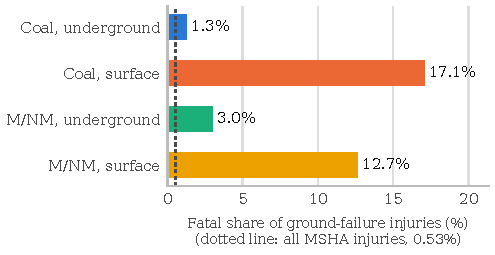
\includegraphics[width=\columnwidth]{figures/paper_cfr.pdf}
\caption{Case-fatality share of ground-failure injuries by setting, 2000--2026. Surface ground-failure injuries are \CFRSurfVsUG{} times as likely to be fatal as underground ones (\CFRSurf\% against \CFRUG\%).}
\label{fig:cfr}
\end{figure}

\paragraph{Exposure-adjusted, surface rates are low} Divided by hours, surface rates are far below underground ones: over 2000--2025 the injury rate was \RateAllCUG{} per 200,000 hours in underground coal and \RateAllMSurf{} at surface metal and nonmetal mines, a ratio of about \RatioUGCoalVsSurfMNM{} to one, on \HoursCUG{} and \HoursMSurf{} billion hours respectively. The fatality rate differs less, about \FRatioUGCoalVsSurfMNM{} to one (\FRateAllCUG{} against \FRateAllMSurf{} per 100 million hours). Both views matter: per hour a surface worker is far safer from ground failure, but when a surface wall does fail, it is far more likely to kill.

\section{Finding 2: Rates Have Fallen Unevenly, and Deaths Have Not Followed Injuries Everywhere}

\begin{figure*}[t]
\centering
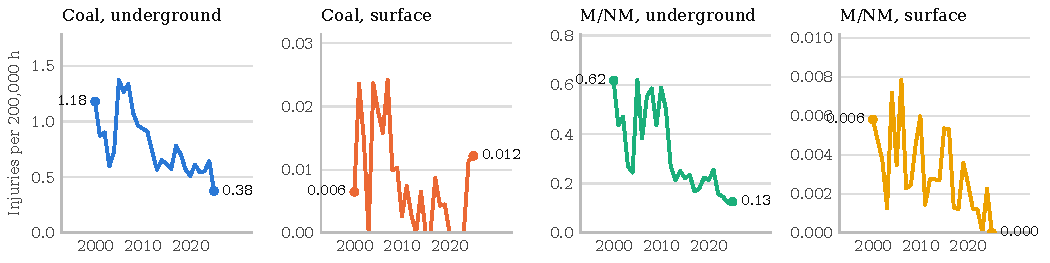
\includegraphics[width=\textwidth]{figures/paper_rates.pdf}
\caption{Ground-failure injury rate per 200,000 hours worked by mine-operator employees, by setting, 2000--2025. Each panel has its own scale; surface rates are two orders of magnitude lower than underground rates. Labels mark the first and last years.}
\label{fig:rates}
\end{figure*}

\paragraph{Injury rates fell in every setting} In underground coal the yearly injury rate fell from \YRateCoalUndergroundTwoZeroZeroZero{} in 2000 to \YRateCoalUndergroundTwoZeroTwoFive{} in 2025, and in underground metal and nonmetal mines from \YRateMNMUndergroundTwoZeroZeroZero{} to \YRateMNMUndergroundTwoZeroTwoFive{} (Figure~\ref{fig:rates}). Pooled into five-year periods to damp year-to-year noise (Table~\ref{tab:periods}), the underground coal rate fell \RateDropCUG\% from 2000--04 to 2020--25, after peaking in 2005--09, and the underground metal and nonmetal rate fell \RateDropMUG\%. Surface rates fell by about three quarters (\RateDropCSurf\% for coal and \RateDropMSurf\% for metal and nonmetal) from much lower levels, on very small counts.

\begin{table}[t]
\small\centering
\setlength{\tabcolsep}{3pt}
\begin{tabular}{@{}lrrrrr@{}}
\toprule
& \textbf{00--04} & \textbf{05--09} & \textbf{10--14} & \textbf{15--19} & \textbf{20--25} \\
\midrule
\multicolumn{6}{@{}l}{\textit{Injuries per 200,000 hours}} \\
\tablefile{tables/periods.tex}
\bottomrule
\end{tabular}
\caption{Ground-failure injury rates (upper block) and fatality rates per 100 million hours (lower block) by five-year period, mine-operator employees.}
\label{tab:periods}
\end{table}

\paragraph{Fatality rates did not follow everywhere} In underground coal the fatality rate fell with the injury rate, from \FRateFirstCUG{} to \FRateLastCUG{} per 100 million hours (\FCountFirstCUG{} and \FCountLastCUG{} deaths; 95\% intervals \FRateLoFirstCUG--\FRateHiFirstCUG{} and \FRateLoLastCUG--\FRateHiLastCUG). In underground metal and nonmetal mines it did not: \FRateFirstMUG{} in 2000--04 and \FRateLastMUG{} in 2020--25 (\FCountFirstMUG{} and \FCountLastMUG{} deaths; intervals \FRateLoFirstMUG--\FRateHiFirstMUG{} and \FRateLoLastMUG--\FRateHiLastMUG), while the injury rate fell by more than half. The intervals overlap, so the data do not show an increase; they show that the decline in injuries has not been matched by a measurable decline in deaths. A falling injury rate with a flat fatality rate is consistent with controls that reduce frequent small falls without reducing rare large ones, and it is the pattern that surveillance by injury counts alone would miss.

\paragraph{Commodity} Among underground metal and nonmetal mines, metal mines have the highest injury rate (\RateUGMetal{} per 200,000 hours, against \RateUGStone{} for stone and \RateUGNonmetal{} for nonmetal), while underground stone mines have the highest fatality rate (\FRateUGStone{} per 100 million hours, against \FRateUGMetal{} for metal). Appendix~D gives every commodity.

\paragraph{Geography} Ground-failure injuries concentrate where underground mining concentrates. \TopThreeCUG{} account for \TopThreeShareCUG\% of underground coal injuries among \NStatesCUG{} states with underground coal hours; among underground metal and nonmetal mines, the top three states account for \TopThreeShareMUG\% across \NStatesMUG{} states. Rates vary as much as counts: Idaho's underground metal and nonmetal mines recorded \InjIDMUG{} injuries at \RateIDMUG{} per 200,000 hours, against \InjNVMUG{} at \RateNVMUG{} in Nevada, which worked several times as many hours. Surface metal and nonmetal injuries are spread thinly across \NStatesMSurf{} states. Appendix~C lists the leading states in every setting.

\section{Finding 3: The Federal Record Rarely Says How Surface Walls Fail}
\paragraph{Mechanism is seldom stated} Of the \NCoded{} surface metal and nonmetal narratives (\ComStone{} stone, \ComMetal{} metal, \ComSandGravel{} sand and gravel, \ComNonmetal{} nonmetal; \NCodedFatal{} fatal), the rules label \ModeRockfall{} as rockfall and \ModeCollapseMechanismUnstated{} as collapse with no mechanism stated (Figure~\ref{fig:modes}, Appendix Table~\ref{tab:modes}). Only \NMechanismNamed{} narratives (\PctMechanismNamed\%) name a structurally controlled mechanism (wedge \ModeWedge, planar \ModePlanar, toppling \ModeToppling, rotational slide \ModeRotationalSlide), and \ModeUnspecified{} (\PctUnspecified\%) match no pattern. The collapse class carries \NCollapseFatal{} of the \NCodedFatal{} deaths: the most lethal events are the ones whose mechanism is least often recorded. Table~\ref{tab:modesq} shows narratives from each class.

\begin{figure}[t]
\centering
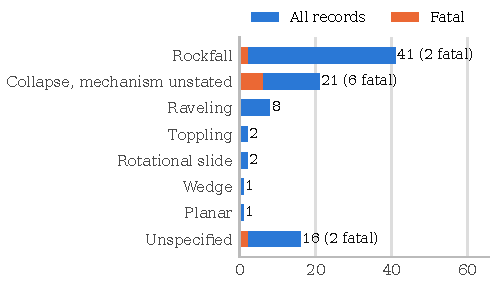
\includegraphics[width=\columnwidth]{figures/paper_modes.pdf}
\caption{Rule-based failure modes of \NCoded{} surface metal and nonmetal ground-failure narratives, 2000--2026, with fatal records overlaid. Rules version \RulesVersion.}
\label{fig:modes}
\end{figure}

\begin{table}[t]
\small
\begin{tabularx}{\columnwidth}{@{}L@{}}
\toprule
\tablefile{tables/quotes_modes.tex}
\bottomrule
\end{tabularx}
\caption{Verbatim MSHA narratives by rule label (commodity, state, year; degree of injury). Narratives are public records, quoted as filed.}
\label{tab:modesq}
\end{table}

When a narrative does describe the mechanism, it can be precise: one operator reported ``multiple geologic faults along the highwall'' acting as release planes for ``a toppling deformation mechanism''. Such reports show that the information exists at the mine. The reporting form simply does not ask for it.

\paragraph{Triggers are seldom recorded} Only \TrigAny{} narratives (\PctTrigAny\%) mention any trigger: blasting \TrigBlasting, water \TrigWater, scaling \TrigScaling. Several describe failures during or just after the work that loads or disturbs a wall: loading blast holes beneath a highwall, cleaning shot rock at the toe, scaling with a rock breaker. The excavator, loader, haul truck, drill, shovel, or dredge appears in \NEquipment{} narratives (\PctEquipment\%), often as the thing struck: equipment working at the toe of a wall is where surface ground failures meet people.

\paragraph{Rule errors found by inspection} Because v1.0 has no formal agreement study, we report the systematic errors we found by reading the labelled narratives (Table~\ref{tab:errors}). The word ``slough'' sends two very large highwall failures, one of about 1.06 million tons across ten benches, to \emph{raveling}, a label meant for progressive small-scale loss. ``Slid'' sends a freeze--thaw rock slide to \emph{planar} without evidence of a sliding plane. The water trigger fires on water as a location (a wall falling into a dredge pond) as well as a cause. And MSHA's fall category itself contains at least one record that is not a ground failure: a stone ejected from a cone crusher. These errors point to specific rule changes (volume thresholds for raveling, requiring a named discontinuity for planar, distinguishing causal from locative water) that we plan for the next version, alongside a blind agreement study.

\begin{table}[t]
\small
\begin{tabularx}{\columnwidth}{@{}L@{}}
\toprule
\tablefile{tables/quotes_errors.tex}
\bottomrule
\end{tabularx}
\caption{Labelling and selection errors found by inspection (rules version \RulesVersion).}
\label{tab:errors}
\end{table}

\paragraph{The classification misses comparable events} Screening the \emph{other} MSHA categories at surface metal and nonmetal mines yields \NCand{} narratives that read as ground failures, \CandRatio{} times the \NCoded{} records selected by MSHA's fall categories, including \NCandFatal{} fatal records (Appendix~E). They are filed mostly as powered haulage (\NCandPH) and machinery (\NCandMach), because the reporting form asks for the circumstance that most directly contributed, and an operator may reasonably name the loader a highwall fell on. Table~\ref{tab:cand} shows examples, including one false positive: the screen is deliberately broad and its output is a review list, not a count. Even if only a fraction are confirmed, surface ground failures are undercounted by any analysis, including ours, that relies on the classification alone.

\begin{table}[t]
\small
\begin{tabularx}{\columnwidth}{@{}L@{}}
\toprule
\tablefile{tables/quotes_candidates.tex}
\bottomrule
\end{tabularx}
\caption{Candidate ground failures filed outside MSHA's fall categories at surface metal and nonmetal mines.}
\label{tab:cand}
\end{table}

\section{Discussion}
GroundFall-US shows a hazard that has receded in frequency but not in lethality. Underground, decades of roof bolting, screen, and rib support have cut injury rates, yet underground metal and nonmetal fatality rates have not fallen with them. At the surface, ground failures are rare per hour worked, but \CFRSurf\% of the injuries they cause are fatal, and the federal record seldom says how the wall failed or what preceded it. Counting injuries alone would understate both problems.

\paragraph{Recommendations} First, MSHA's Part 50 reporting could add a small set of structured fields for ground-failure events: failure mode (from a short list such as the one used here), approximate volume or dimensions, wall or bench height, and observed precursors or triggers (blast, rain, freeze--thaw, scaling, undercutting). Operators already know these facts, as the most detailed narratives show; recording them in fields rather than free text would make national analysis routine. Second, any classification-based count of surface ground failures should be paired with a narrative screen like ours, because the circumstance code alone misses events. Third, the low-frequency, high-severity profile of surface failures argues for investment in monitoring (radar, prism, and visual inspection programs under 56.3130) at walls where equipment works at the toe, which is where the narratives place most victims. GroundFall-US offers a baseline against which such programs can be evaluated.

\paragraph{Future work} The next version will add a blind agreement study of the coding rules, expert review of the \NCand{} candidates, the rule changes identified above, and historical rather than current mine attributes. The same pipeline extends naturally to underground narratives, where rib and roof falls could be coded by support condition.

\paragraph{Conclusion} We released an open, documented, reproducible dataset of \NGF{} ground-failure records at U.S. mines from 2000 to 2026, with rates per hour worked and a transparent failure-mode coding layer. Ground failures cause \PctGFofFatal\% of mining deaths in MSHA's record; surface failures are \CFRSurfVsUG{} times as lethal per injury as underground ones; injury rates have fallen faster than fatality rates in underground metal and nonmetal mining; and the federal record rarely captures failure mechanism or trigger. We offer the dataset as a national reference for MSHA, NIOSH, operators, and researchers, and as the evidence base for early warning.

\section{Data and Code Availability}
Data, code, coding rules, documentation, and the three source files are at \url{https://github.com/Lookman1234/groundfall-us} (release v1.0.0), and will be archived on Zenodo with a DOI at release. Data and documentation are licensed CC BY 4.0 and code MIT. The README gives the commands to rebuild every table and figure; the source fingerprints are in Appendix~F.

\section{Acknowledgments}
We thank the Mine Safety and Health Administration for maintaining its open data portal.

\section{Ethics Statement}
This study uses only public administrative records. MSHA publishes accident narratives, mine identifiers, and operator names as open government data; the narratives contain no worker names, and we quote them verbatim, as filed, identifying each by commodity, state, and year only. We made no contact with mines, operators, or workers. Narratives describe injuries and deaths of real people; we quote them to document the hazard and the limits of the record, not to assign fault, and nothing here is a finding about the conduct of any operator.

\paragraph{Use of AI assistance} Code for fetching, joining, and analysing the data, the initial draft of the coding rules, and drafting of this manuscript were assisted by an AI system (Claude, Anthropic). The authors directed the work, made the analytic decisions, approved the coding rules, and are responsible for the content. Every number in the paper is generated by the released code from the released data.

\paragraph{Positionality} The coding rules reflect the judgment of the first author, who wrote them. Rules written by a different expert might draw some boundaries differently, which is why every rule and the evidence phrase behind every label are released for inspection.

\begin{thebibliography}{99}
\bibitem[{Coleman and Kerkering(2007)}]{ColemanKerkering2007}
Coleman, P.~J.; and Kerkering, J.~C. 2007.
\newblock Measuring Mining Safety with Injury Statistics: Lost Workdays as Indicators of Risk.
\newblock \emph{Journal of Safety Research}, 38(5): 523--533.

\bibitem[{Code of Federal Regulations(2026a)}]{CFRPart50}
Code of Federal Regulations. 2026a.
\newblock 30 CFR Part 50: Notification, Investigation, Reports and Records of Accidents, Injuries, Illnesses, Employment, and Coal Production in Mines.
\newblock \url{https://www.ecfr.gov/current/title-30/part-50}.

\bibitem[{Code of Federal Regulations(2026b)}]{CFR563130}
Code of Federal Regulations. 2026b.
\newblock 30 CFR 56.3130: Wall, Bank, and Slope Stability.
\newblock \url{https://www.ecfr.gov/current/title-30/section-56.3130}.

\bibitem[{Friedman et~al.(2015)}]{Friedman2015}
Friedman, L.; Swedler, D.; Almberg, K.; and Cohen, R. 2015.
\newblock Evaluation of the Completeness of Injury and Illness Reporting in the Illinois Mining Industry: Comparing Workers' Compensation Claims to the MSHA Part 50 Program.
\newblock Final Report, University of Illinois at Chicago School of Public Health, for the U.S. Department of Labor Chief Evaluation Office.

\bibitem[{Ganguli, Miller, and Pothina(2021)}]{Ganguli2021}
Ganguli, R.; Miller, P.; and Pothina, R. 2021.
\newblock Effectiveness of Natural Language Processing Based Machine Learning in Analyzing Incident Narratives at a Mine.
\newblock \emph{Minerals}, 11(7): 776.

\bibitem[{Gebru et~al.(2021)}]{Gebru2021}
Gebru, T.; Morgenstern, J.; Vecchione, B.; Vaughan, J.~W.; Wallach, H.; Daum\'e~III, H.; and Crawford, K. 2021.
\newblock Datasheets for Datasets.
\newblock \emph{Communications of the ACM}, 64(12): 86--92.

\bibitem[{Goodman and Bray(1976)}]{GoodmanBray1976}
Goodman, R.~E.; and Bray, J.~W. 1976.
\newblock Toppling of Rock Slopes.
\newblock In \emph{Rock Engineering for Foundations and Slopes: Proceedings of the ASCE Specialty Conference}, volume~2, 201--234. Boulder, Colorado: ASCE.

\bibitem[{Groves, Kecojevic, and Komljenovic(2007)}]{Groves2007}
Groves, W.~A.; Kecojevic, V.~J.; and Komljenovic, D. 2007.
\newblock Analysis of Fatalities and Injuries Involving Mining Equipment.
\newblock \emph{Journal of Safety Research}, 38(4): 461--470.

\bibitem[{Hungr, Leroueil, and Picarelli(2014)}]{Hungr2014}
Hungr, O.; Leroueil, S.; and Picarelli, L. 2014.
\newblock The Varnes Classification of Landslide Types, an Update.
\newblock \emph{Landslides}, 11(2): 167--194.

\bibitem[{Khademian et~al.(2022)}]{Khademian2022}
Khademian, Z.; Rashed, G.; Sears, M.; and Xue, Y. 2022.
\newblock Ground-Fall Accident Trends in Mining: 2010 to 2019.
\newblock In \emph{Proceedings of the 41st International Conference on Ground Control in Mining}, 1--20. Canonsburg, Pennsylvania: SME.

\bibitem[{Mark, Pappas, and Barczak(2009)}]{MarkPappasBarczak2009}
Mark, C.; Pappas, D.~M.; and Barczak, T.~M. 2009.
\newblock Current Trends in Reducing Groundfall Accidents in U.S. Coal Mines.
\newblock SME Annual Meeting, Preprint 09-069. Denver, Colorado: Society for Mining, Metallurgy, and Exploration.

\bibitem[{Mine Safety and Health Administration(2026)}]{MSHAOGD}
Mine Safety and Health Administration. 2026.
\newblock Open Government Data: Accident Injuries, Mines, and Employment/Production (Yearly) Data Sets, Edition of 9 October 2026.
\newblock \url{https://arlweb.msha.gov/OpenGovernmentData/OGIMSHA.asp}.

\bibitem[{Pappas and Mark(2012)}]{PappasMark2012}
Pappas, D.~M.; and Mark, C. 2012.
\newblock Roof and Rib Fall Incident Trends: A 10-Year Profile.
\newblock \emph{Transactions of the Society for Mining, Metallurgy, and Exploration}, 330: 462--478.

\bibitem[{Read and Stacey(2009)}]{ReadStacey2009}
Read, J.; and Stacey, P., eds. 2009.
\newblock \emph{Guidelines for Open Pit Slope Design}.
\newblock Melbourne: CSIRO Publishing.

\bibitem[{Varnes(1978)}]{Varnes1978}
Varnes, D.~J. 1978.
\newblock Slope Movement Types and Processes.
\newblock In \emph{Landslides: Analysis and Control}, Special Report 176, 11--33. Washington, DC: Transportation Research Board.

\bibitem[{Wilkinson et~al.(2016)}]{Wilkinson2016}
Wilkinson, M.~D.; Dumontier, M.; Aalbersberg, I.~J.; et~al. 2016.
\newblock The FAIR Guiding Principles for Scientific Data Management and Stewardship.
\newblock \emph{Scientific Data}, 3: 160018.

\bibitem[{Wyllie and Mah(2004)}]{WyllieMah2004}
Wyllie, D.~C.; and Mah, C.~W. 2004.
\newblock \emph{Rock Slope Engineering: Civil and Mining}.
\newblock 4th edition. London: Spon Press.
\end{thebibliography}

\clearpage
\onecolumn
\section*{Appendix A: Codebook (Incident Table)}
\begin{table}[H]
\small
\begin{tabularx}{\textwidth}{@{}llL@{}}
\toprule
\textbf{Column} & \textbf{Source} & \textbf{Definition} \\
\midrule
\texttt{document\_no} & Accidents & MSHA accident form number; unique key. \\
\texttt{mine\_id} & Accidents & Seven-digit MSHA mine identifier. \\
\texttt{mine\_name}, \texttt{state}, \texttt{county}, \texttt{latitude}, \texttt{longitude} & Mines & Current mine name and location. \\
\texttt{accident\_date}, \texttt{year} & Accidents & Date of the event and calendar year. \\
\texttt{sector} & Derived & Coal or metal/nonmetal, from \texttt{COAL\_METAL\_IND}. \\
\texttt{subunit\_cd}, \texttt{subunit}, \texttt{mine\_type} & Accidents, derived & Location within the mine and grouped mine type (underground, surface, mill/plant, shop/yard, office). \\
\texttt{commodity}, \texttt{primary\_sic} & Mines & Grouped canvass (coal, metal, nonmetal, stone, sand and gravel) and SIC description. \\
\texttt{msha\_classification} & Accidents & MSHA circumstance category (selection variable). \\
\texttt{degree\_injury\_cd}, \texttt{severity} & Accidents, derived & Degree of injury and grouped severity (fatal, lost time, other reportable injury, no-injury accident, other). \\
\texttt{is\_fatal}, \texttt{is\_injury}, \texttt{is\_lost\_time} & Derived & Flags from the degree of injury. \\
\texttt{is\_contractor}, \texttt{contractor\_id} & Accidents & Contractor involvement. \\
\texttt{occupation}, \texttt{activity}, \texttt{mining\_equipment} & Accidents & As reported. \\
\texttt{has\_hours\_same\_year} & Derived & Hours exist for the same mine, subunit, and year. \\
\texttt{narrative} & Accidents & Operator narrative, as filed. \\
\bottomrule
\end{tabularx}
\caption{Incident-table columns. The rate table adds hours, average employees, counts by severity, and rates; the failure-mode table adds \texttt{failure\_mode}, trigger flags, and the evidence phrase for each label. Full definitions are in \texttt{docs/CODEBOOK.md}.}
\end{table}

\section*{Appendix B: Coding Rules (Version \RulesVersion)}
\begin{table}[H]
\small
\begin{tabularx}{\textwidth}{@{}lrL@{}}
\toprule
\textbf{Label (in precedence order)} & \textbf{Patterns} & \textbf{First pattern (regular expression) and exclusion} \\
\midrule
\tablefile{tables/rules.tex}
\bottomrule
\end{tabularx}
\caption{Coding rules. Modes are tested in the order listed and the first match wins; triggers are independent. The full rule set is \texttt{config/coding\_rules.yaml}.}
\end{table}

\begin{table}[H]
\small\centering
\begin{tabular}{@{}lrrr@{}}
\toprule
\textbf{Failure mode} & \textbf{Records} & \textbf{\%} & \textbf{Fatal} \\
\midrule
\tablefile{tables/modes.tex}
\bottomrule
\end{tabular}
\caption{Failure-mode distribution, surface metal and nonmetal ground failures, 2000--2026 (n = \NCoded).}
\label{tab:modes}
\end{table}

\section*{Appendix C: Leading States}
\begin{table}[H]
\small
\begin{tabularx}{\textwidth}{@{}lrrL@{}}
\toprule
\textbf{Setting} & \textbf{States} & \textbf{Top-3 \%} & \textbf{Five states with most injuries: count (rate per 200,000 hours, underground only)} \\
\midrule
\tablefile{tables/states.tex}
\bottomrule
\end{tabularx}
\caption{Ground-failure injuries by state, mine-operator employees, 2000--2025. ``States'' counts states with hours worked in the setting.}
\end{table}

\section*{Appendix D: Commodities}
\begin{table}[H]
\small\centering
\begin{tabular}{@{}llrrrrr@{}}
\toprule
\textbf{Commodity} & \textbf{Type} & \textbf{Hours (millions)} & \textbf{Injuries} & \textbf{Deaths} & \textbf{Injury rate} & \textbf{Fatality rate} \\
\midrule
\tablefile{tables/commodity.tex}
\bottomrule
\end{tabular}
\caption{Ground-failure injuries and deaths by commodity and mine type, mine-operator employees, 2000--2025. Injury rate per 200,000 hours; fatality rate per 100 million hours. Settings with under one million hours are omitted.}
\end{table}

\section*{Appendix E: Supplement Candidates by MSHA Category}
\begin{table}[H]
\small\centering
\begin{tabular}{@{}lrr@{}}
\toprule
\textbf{MSHA classification} & \textbf{Candidates} & \textbf{Fatal} \\
\midrule
\tablefile{tables/candidates.tex}
\bottomrule
\end{tabular}
\caption{Surface metal and nonmetal narratives outside MSHA's fall categories flagged by the screen (n = \NCand), 2000--2026. Candidates await expert review and are not in the v1.0 counts.}
\end{table}

\section*{Appendix F: Reproducibility}
The pipeline runs in eight numbered scripts (fetch, build, QA, coding, candidate screen, validation sample, figures, summary) plus the script that generates every number in this paper. Run with the archived source files, it reproduces every table byte for byte; we verified this with an independent rebuild. Source files and fingerprints:
\begin{table}[H]
\small\centering
\begin{tabular}{@{}lrp{3.6in}@{}}
\toprule
\textbf{File} & \textbf{Bytes} & \textbf{SHA-256} \\
\midrule
\tablefile{tables/provenance.tex}
\bottomrule
\end{tabular}
\caption{MSHA source files, edition of 9 October 2026.}
\end{table}

\end{document}
